Comme vu précédemment, la démocratisation de l'électronique puis de l'informatique au XXème siècle n'a eu de cesse de faire émerger de nouvelles pratiques compositionnelles.
Cette section présente succinctement les catégories d'outils informatiques qui, de nos jours, sont des pierres angulaires de la création musicale. Le but est de décrire l'environnement informatique dans lequel évolue les compositeurs et qui influence de fait leur mode de composition, donc de notation de la musique. 

\subsection{Stations audionumériques}
\label{subsec:stationAudionum}
Une station audionumérique désigne un \og ensemble d'outils électroniques, conçu pour enregistrer, éditer, manipuler, créer et lire des contenus audionumériques \fg (Wikipédia).
Les logiciels employés dans le cadre de l'édition de contenu audionumérique sont également qualifiés de stations audionumériques.
Les logiciels Pro Tools (Avid), Ableton Live (Ableton Inc.), ou encore Ardour (open-source porté par Paul Davis) peuvent être cités comme exemples.
Ces programmes possèdent une interface similaire : Plusieurs pistes placées sur une ligne de temps contiennent des fichiers audio, présentés en forme d'ondes, ou des instructions MIDI, présentés en \textit{piano roll}\footnote{Le \textit{piano roll}, dans son acception moderne, est un mode de visualisation et d'édition de notes MIDI, inspiré des rouleaux de papier perforé autrefois utilisés dans les pianos mécaniques. Les touches du piano sont représentés sur l'axe vertical, et la ligne du temps sur l'axe horizontal. Une note MIDI est représenté dans la grille par un rectangle de longueur variable.}. Comme exemple, l'interface graphique du logiciel \textit{Ardour} est présentée en figure \ref{fig:exempleDaw}. 

\begin{figure}[H]
	\centering
	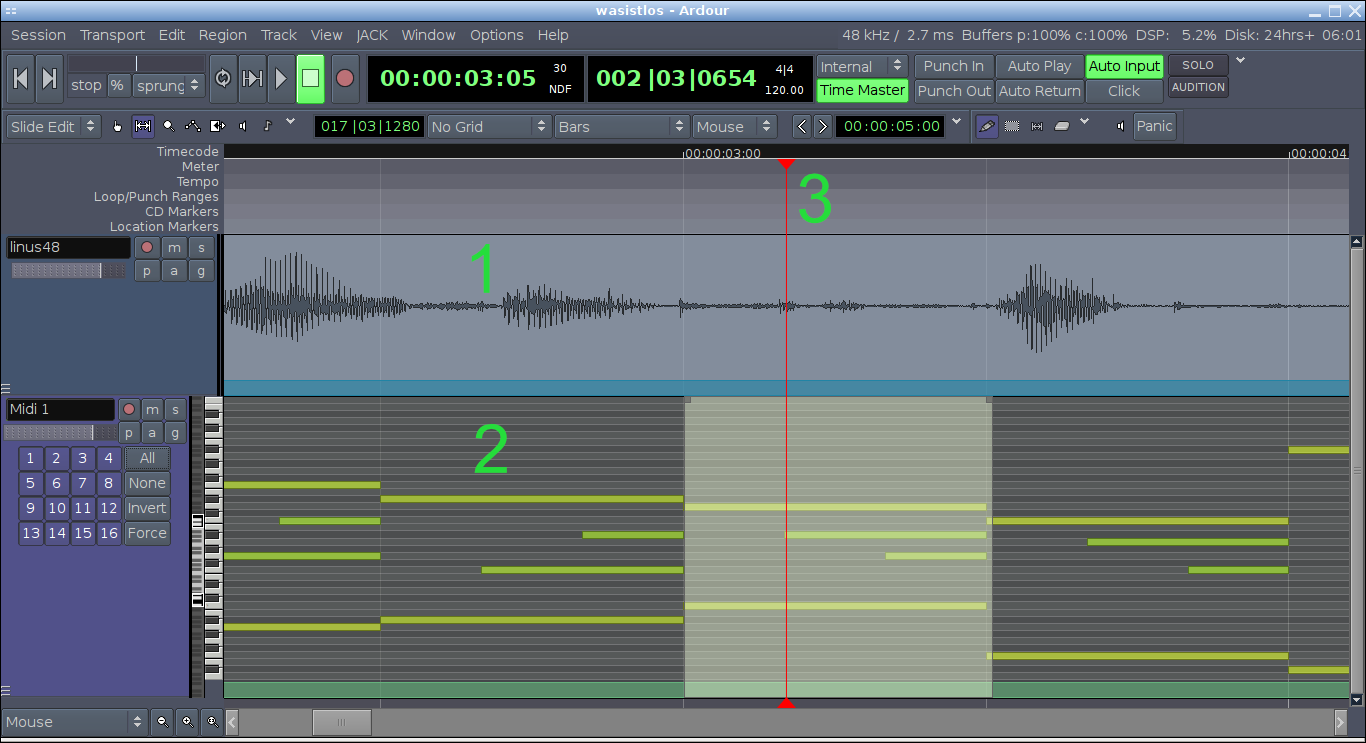
\includegraphics[keepaspectratio=true, width=0.8\textwidth]{OutilsInformatiques/i/exempleDaw.png}
	\caption{Interface graphique de la station audionumérique Ardour}
	\label{fig:exempleDaw}
	\small
	\it
	En 1, une piste audio avec une représentation du son en forme d'ondes. En 2, une piste MIDI visualisée sous forme de piano roll. En 3, la barre de lecture.					
\end{figure}

Certains paramètres associés à une piste (volume, panoramique, réverbération…) peuvent être automatisés et visualisés sous formes de courbes de variations au-dessus ou en-dessous du contenu de la piste. La figure \ref{fig:exempleAutomation} présente une vue de courbes d'automation décrites avec le logiciel Ardour.

\begin{figure}[H]
	\centering
	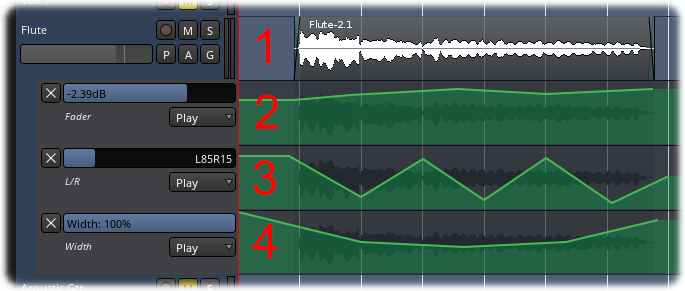
\includegraphics[keepaspectratio=true, width=0.7\textwidth]{OutilsInformatiques/i/exempleAutomation.png}
	\caption{Courbes d'automation pour trois paramètres d'une piste}
	\label{fig:exempleAutomation}
	\small
	\it
	En 1, la piste Flute et son contenu audio. En 2, 3 et 4, trois courbes d'automation pour les paramètres de volume, panoramique et largeur stéréo de la piste Flute.					
\end{figure}

De fait, l'interface graphique d'une station audionumérique présente assez d'informations visuelles pour décrire le contenu audio, faisant d'elle une potentielle \og partition \fg.
Cependant, le manque de symbolisme des représentations empêche une réelle compréhension ou audition de la musique à travers une telle interface \cite{gottfried2017}.

\subsection{Langages de programmation visuelle pour la création musicale}
\label{subsec:programmationVisuelle}
Un langage de programmation visuelle ou graphique \og permet à un utilisateur de spécifier un programme dans un mode bi ou multidimensionnel \fg \cite{myers1989}. A savoir, ces langages proposent des éléments visuels autres que le simple texte pour manipuler les concepts et structures propres à la programmation informatique. Aussi, leur caractère graphique facilite leur prise en main par les non-informaticiens \cite{bresson2009}.
De fait, l'apparition d'environnements de programmation visuelle dédiés à la création musicale répond à un besoin des compositeurs de disposer de langages informatiques pour la génération de processus musicaux    

Les langages visuels de production musicale peuvent être séparés en deux catégories. La première catégorie regroupe les langages permettant le calcul de structures musicales et sonores en \og temps différé \fg. La deuxième catégorie implique les environnements prenant en compte l'interactivité avec l'utilisateur lors d'une exécution temps-réel.

\paragraph{Langages de composition temps différé} Un des premiers langages de composition assistée par ordinateur (temps différé) est PatchWork (\textit{PW}), développé par Mikael Laurson \cite{laurson1989}. PW est construit au-dessus du langage Common Lisp. Une version de PW utilisant la librairie OpenGL pour le rendu graphique, nommé PWGL a ensuite était implémentée \cite{laurson2002}. 

OpenMusic (\textit{OM}), un autre successeur de PW, est un langage créé et développé à l'IRCAM \cite{agon1998, assayag1999}. OpenMusic est toujours activement maintenu et utilisé par les compositeurs de musique contemporaine; il sera donc pris en exemple pour expliquer les caractéristiques des langages orientés exécution à la demande.
Comme pour PW, OpenMusic est basé sur le langage Common Lisp, et peut être considéré comme un \textit{front-end} graphique de Lisp \cite{bresson2009}. OM permet de définir des \textit{patches}, qui sont des diagrammes représentant une unité fonctionnelle du langage. Un patch OM regroupe un ensemble de \textit{boîtes}, matérialisant des fonctions (primitives ou définies par l'utilisateur) ou des constructeurs d'objets accompagnés d'éditeur graphique. De nombreux objets et fonctions pour la création musicale sont nativement intégrés; par exemple, les objets \textit{chord}, \textit{note}, \textit{voice}, ou les fonctions de manipulation du format MIDI… Chaque boîte possède un ensemble de points d'entrée et de sortie, symbolisant respectivement ses paramètres et sa(ses) valeur(s) de retour. Des connexions, sous de formes de cordes, peuvent être établies entre deux boîtes en reliant les valeurs de sorties de l'une aux entrées de l'autre. De fait, un patch OM peut être vu comme un graphe orienté acyclique partant d'un élément racine, l'élément le plus bas du diagramme, jusqu'aux éléments les plus hauts. La figure \ref{fig:exempleOpenMusic} montre un exemple de patch OpenMusic computant une structure musicale.

\begin{figure}[H]
	\centering
	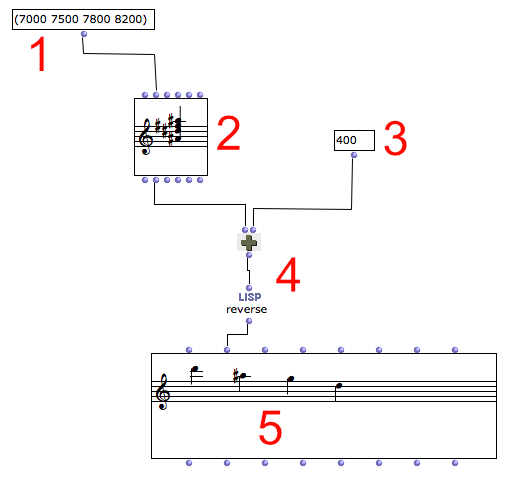
\includegraphics[keepaspectratio=true, width=0.5\textwidth]{OutilsInformatiques/i/exempleOpenMusic.png}
	\caption{Patch OpenMusic générant une séquence de notes à partir d'un accord}
	\label{fig:exempleOpenMusic}
	\small
	\it
	En 1, une liste d'entiers en syntaxe Lisp. En 2, un objet \textbf{chord} (accord) recevant la liste 1 en paramètre comme définition de la hauteur des notes. En 3, un simple littéral entier, deuxième argument passé à la méthode \textbf{om+} (l'icône +). Ici, la méthode \textbf{om+} va effectuer l'addition entre 400 et chaque élément de la liste en 1, puis retourner la liste résultante. En 4, la fonction Lisp \textbf{reverse} inverse l'ordre de la liste passée en entrée. En 5, l'objet \textbf{chord-seq} affiche la liste inversée sous forme d'une séquence de notes.	
\end{figure}

Pour évaluer un patch, c'est à dire calculer sa valeur de sortie, la racine du patch va demander récursivement aux boîtes dont la sortie est liée à ses entrées de s'évaluer. Lorsque la racine a déterminé la valeur de ses paramètres, elle s'évalue elle-même et retourne son résultat.
Aussi, un patch peut être utilisé dans un autre patch comme une simple boîte fonctionnelle, demandant des entrées et fournissant des sorties.
Les types de langages comme OM et PW sont dits orientés \og exécution à la demande \fg (\textit{demand-driven execution}) car l'interprétation d'un patch n'est pas soumise à une contrainte temporelle. Ces outils de composition assistée par ordinateur s'inscrivent dans la même temporalité que celle du compositeur préparant sa pièce\footnote{Cependant, une nouvelle version de OM, appelée \textit{O7}, étend le comportement du langage vers plus d'interactivité avec l'utilisateur au moment de l'interprétation \cite{bresson2017}.}.
En particulier, les éditeurs de notation musicale y sont des points d'entrées et de sortie privilégiés pour la création et l'exécution de processus musicaux \cite{kuuskankare2006, }. 
   

\paragraph{Langages orientés gestion du temps réel} Le langage Max/MSP est un pionnier, d'abord en termes de programmation visuelle dédiée aux applications musicales, ensuite en termes de capacité de traitement et de génération du signal audio en temps réel \cite{favreau1986}\footnote{PureData est un autre langage visuel open-source pour l'interaction temps-réel répondant aux mêmes principes que Max \cite{puckette1996}.}.
Sur le même mode que pour OpenMusic, l'unité programmationnel de Max/MSP est le patch. Un patch Max est également constitué de boîtes avec entrées et sorties reliées entre elles par des cordes. En revanche, l'interprétation d'une boîte Max ne se fait pas sur le même mode. Un patch Max est soit en mode édition (\textit{edit mode}), pendant lequel de nouvelles boîtes peuvent être ajoutées, déplacées, connectées, soit en mode exécution (\textit{run mode}), alors l'utilisateur ne peut interagir qu'avec les boîtes de contrôle (boutons, sliders…) \cite{puckette1991}. Les boîtes Max communiquent entre elles via l'envoi de messages. Un message est toujours envoyé depuis la sortie d'une boîte vers l'entrée d'une autre boîte. Le contenu d'un message peut être de plusieurs types (entier, chaîne de caractères, liste, objet complexe…); le message \textit{signal} est une particularité \cite{max2018}. En effet, les objets Max dont le nom fini par $\sim$ sont responsables de l'envoi ou de la réception de messages de type signal. Un objet $\sim$ envoie (en mode exécution) un message de type signal régulièrement à sa sortie, selon une valeur cyclique interne à Max, pour simuler un flot continuel de données. La figure \ref{fig:exempleMax} donne un exemple de patch Max/MSP produisant une fréquence sonore. Les liaisons portant des signaux sont en pointillés.

\begin{figure}[H]
	\centering
	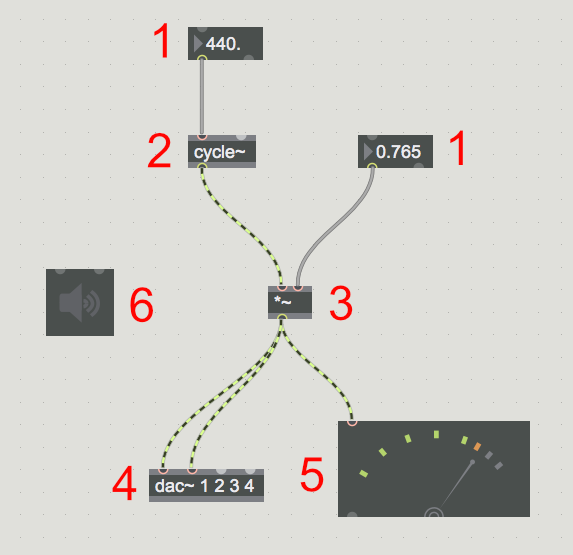
\includegraphics[keepaspectratio=true, width=0.5\textwidth]{OutilsInformatiques/i/exempleMax.png}
	\caption{Patch Max/MSP produisant une fréquence sinusoïdale de 440Hz}
	\label{fig:exempleMax}
	\small
	\it
	En 1, deux \emph{number boxes} qui envoient un message à chaque changement de leur valeur. En 2, l'objet \emph{cycle$\sim$} qui envoie un message de type signal correspondant à une onde sinusoïdale de fréquence spécifiée en entrée (ici 440Hz). En 3, \emph{*$\sim$} qui renvoie le signal résultant de la multiplication entre le signal reçu de \emph{cycle$\sim$} et le coefficient du slider. En 4, l'objet \emph{dac$\sim$} gérant la sortie sur le périphérique audio. En 5, l'objet \emph{levelmeter} pour une visualisation de l'intensité du signal reçu. En 6, l'objet \emph{ezdac$\sim$} activant ou désactivant la sortie audio.			
\end{figure}

 Pendant longtemps, le traitement et la production de signal audio ont été les principales tâches qui pouvaient être accomplies avec Max/MSP. Récemment, la librairie \textit{bach} a apporté au langage des éléments permettant la composition assistée par ordinateur dans un paradigme temps-réel \cite{agostini2013}. \textit{bach} propose deux types de visualisation d'une partition : une vue classique en temps mesuré avec le module bach.score, et une vue en piano-roll en temps linéaire avec le module \textit{bach.roll}. Une extension de \textit{bach}, la librairie \textit{dada} apporte de nombreuses notations alternatives pour l'écriture de la musique \cite{agostini2017}. L'annexe \ref{sec:exempleBachDada} présente les différentes vues de partitions proposées par \textit{bach}.   

\subsection{Interopérabilité}
\label{subsec:interoperabilite}
Afin de faire communiquer différentes applications ou machines impliquer dans un processus de création musicale ou multimédia, plusieurs protocoles et formats d'échange ont été standardisés.

\paragraph{MIDI} Le protocole MIDI (Musical Instrument Digital Interface) a été spécifié pour la première fois en 1982 par l'\textit{International MIDI Association} \cite{international1983}. Aujourd'hui, le protocole MIDI est  largement utilisé par les équipements et logiciels grand public à visée musicale. Ce protocole vise la communication d'informations entre divers systèmes numériques : synthétiseurs, ordinateurs, lecteurs audio… L'unité de transmission du protocole MIDI est le message, composé d'un octet statut et un ou deux octets de données. Le statut décrit le type du message, relevant des catégories \textit{channel} ou \textit{system}. Les messages de la catégorie \textit{channel} décrivent les notes et actions à exécuter par le receveur. Les messages de la catégorie \textit{system} encapsulent des évènements et informations plus généraux, notamment concernant la synchronisation des différents receveurs (\textit{MIDI Time Code}, \textit{System Real Time messages}) \cite{midi1996}.
 
\paragraph{Open Sound Control} Le protocole \textit{Open Sound Control} (OSC) a été spécifié en 2002 au CNMAT de l'Université de Berkeley \cite{wright2002}. OSC propose un format de communication entre processus, ordinateurs, synthétiseurs et autres appareils. Moins démocratisé que MIDI, l'intégration de ce protocole dans différentes programmes, comme Max/MSP, lui donne une visibilité certaine.
L'unité de transmission du protocole OSC est le \textit{paquet OSC}, envoyé dans une même trame UDP ou TCP.
Un paquet OSC contient un \textit{bundle OSC} qui est lui même une composition de messages OSC.
Un bundle OSC regroupe une ensemble de messages devant être interprétés au même moment. De fait, un bundle OSC est associé à une estampille temporelle (\textit{time-tag}), définissant le moment de l'interprétation.
Quant à un message OSC, c'est un simple couple \lstinline[language=html]|<oscaddress>:<value>|, où une \textit{osc-address} est une URI (Unique Resource Identifier) exprimée sous forme de chemin, par exemple \texttt{/synthetizer/2/freq}, et \textit{value} est une valeur de type int, float, string ou blob. 
Une processus envoyant des paquets OSC est qualifié de client OSC et un processus recevant des paquets OSC est qualifié de serveur OSC. Le serveur OSC a la responsabilité de n'interpréter les messages contenus dans un bundle OSC qu'au moment spécifié par l'estampille temporelle associée.

Dans l'environnement Max/MSP, la librairie \textit{o.} (lire \og oh dot \fg) augmente les possibilités fournies par le protocole OSC en lui adjoignant un langage de programmation. \textit{o.} propose un ensemble d'objets Max, préfixés par \og o. \fg (o.build, o.call…), qui génèrent et manipulent des bundles OSC \cite{maccallum2011}.